%%%%
\section{Poluição do Ar}

Poluição do ar resulta de uma complexa mistura de emissões naturais e 
antropogênicas, estima-se que a poluição do ar é responsável por 
$3,2$ milhões de mortes por ano no mundo todo \citep{lim2013}.

A inalação de material particulado $MP$ exerce um papel importante na 
exacerbação de doenças respiratórias, incluindo enfisema pulmonar e asma. 
Suas pequenas dimensões e massa, facilitam a penetração do $MP$ no sistema 
respiratório. 

A deposição no sistema respiratório humano ocorre em função do diâmetro da partícula.
As partículas grossas $MP_{2,5-10}$ ficam retidas no nariz (nasofaringe) e
as partículas mais finas $MP_{2,5}$ chegam nos alvéolos pulmonares e nos bronquíolos.
Nas áreas danificadas ocorre o comprometimento das trocas gasosas podendo, 
também, acarretar problemas cardiovasculares.
O próprio corpo consegue remover partículas através do Macrófago alveolar 
e do sistema linfático. \citep{arbex2012}.

Os vírus são $MP_{2,5}$ e bactérias são $MP_{10}$, 
o que significa que vírus tem maior penetração.

%%%%
\subsection{Material Particulado $MP$}

Material Particulado $MP$ ou Aerossóis Atmosféricos são partículas
sólidas ou líquidas em suspensão em um gás, as quais tem diâmetro 
aerodinâmico compreendido  entre $0,001-100\mu m$. 
A parte considerada inalável para humanos tem diâmetro menor que 10 $\mu m$
e se comporta praticamente como gás.
As partículas maiores que 10 $\mu m$ têm dificuldade em penetrar 
no sistema respiratório porque seu arraste pelo ar inalado não vence 
a força da gravidade \citep{seinfeld1998}.

O $MP$ pode ser classificado por tamanho, formação 
(primária ou secundária), pela forma de remoção da atmosfera, 
composição química ou forma geométrica da partículas \citep{seinfeld1998}.

A divisão por tamanho separa o $MP$ menor de $10 \mu m$ em quatro modas:
ultra-finas, núcleos de Aitken, acumulação e grossa. 

\begin{itemize}
  \item \textbf{ultra-finas:} formada por vapores de baixa votatilidade;
  \item \textbf{nucleação ou núcleos de Aitken:} 
        gerada a partir da condensação de vapores quentes ou durante o processo de 
        transformação de gás em partícula. Partículas formadas por 
        nucleação são removidas da atmosfera por aglomeração.   
  \item \textbf{moda acumulação:} 
         partículas na moda de acumulação são criadas 
         a partir de núcleos de condensação (núcleos de Aitken) através da 
         coagulação ou condensação de vapores. 
         Partículas formadas por acumulação
         são removidas da atmosfera por deposição seca ou úmida.
  \item \textbf{moda grossa ($MP_{2,5-10}$):} 
        são oriundas de processos mecânicos como fragmentação, 
        movimentação e manuseio. Partículas grossas são removidas da atmosfera 
        por sedimentação.
\end{itemize}

A figura proposta por \citep{finlayson1999} ilustra os processos de 
formação e remoção de cada moda. 

\begin{figure}[H]
\begin{center}
  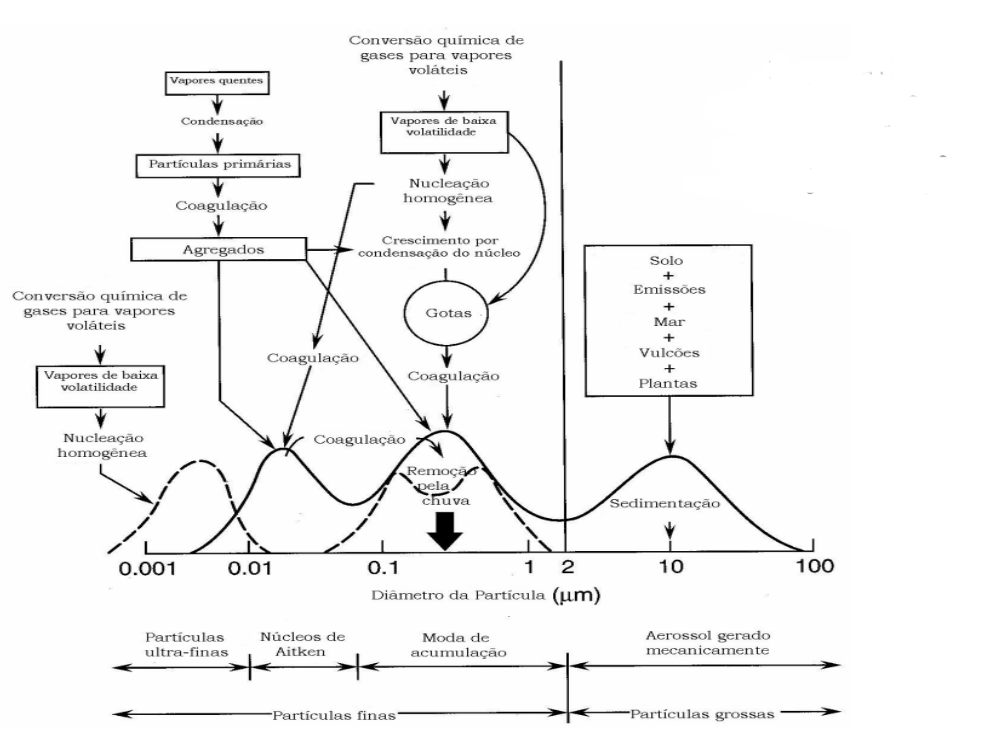
\includegraphics[width=0.8\textwidth]{../inputs/images/modas_aerossol.png}
  \caption{Esquema da distribuição de tamanho do aerossol atmosférico 
           \citep{finlayson1999} \label{fig:modas_aerossol}}
\end{center}
\end{figure}

O material particulado fino $MP_{2,5}$ engloba as partículas 
ultra-finas, a moda de nucleação e a moda de acumulação.  

O $MP_{2,5-10}$ tende a ficar retido na parte superior do sistema respiratório, 
enquanto que $MP_{2,5}$ tem maior facilidade para penetrar e atingir 
os alvéolos pulmonares e corrente sanguínea, 
podendo comprometer significativamente a saúde humana. 

O $MP$ pode ser emitido por diferentes fontes antropogênicas ou naturais e, 
também, pode ser gerado secundariamente na atmosfera, através de 
reações químicas, por exemplo. 

O $MP_{2,5}$ representa uma ameça a saúde humana, pois além 
do alto poder de penetração no sistema respiratório humano,
é gerado pelo processo de conversão gás-partícula, sendo esses 
gases muitas vezes tóxicos.

No $MP_{2,5}$ encontra-se principalmente íons $SO_4^=$, 
íons $ NO_3^-$, carbono elementar, carbono orgânico, 
elementos traços como metais 
(cádmio, níquel, vanádio, zinco, cromo, ferro, mercúrio), 
sulfatos e nitratos \citep{finlayson1999}. 

Compostos como nitrato e sulfato de amônio são poluentes secundários,
pois óxido de nitrogênio $NO_x$ e amônia $NH_3$ formam nitrato de amônio. 
Dióxido de enxofre $SO_2$ e amônia $NH_3$ formam o sulfato de amônio. 

Na moda grossa $MP_{2,5-10}$ há poluentes formados por processos mecânicos, 
como poeira de solo, fuligem, polens, metais alcalinos, entre outros. 

%%%%
%\subsection{Meio Ambiente}
%Ao depositar em folhas, as partículas impedem a absorção de luz. 
%Efeitos na visibilidade.
%Efeitos na formação de nuvens.


